\documentclass{standalone}

\usepackage{amsmath}
\usepackage{tikz, ifthen}
\usetikzlibrary{decorations.pathmorphing,patterns,arrows,decorations.pathreplacing,shapes}

\tikzset{snake it/.style={decorate, decoration={snake, amplitude=0.3mm, segment length=2mm}}}

\definecolor{mygreen}{RGB}{0,100,0}

\begin{document}

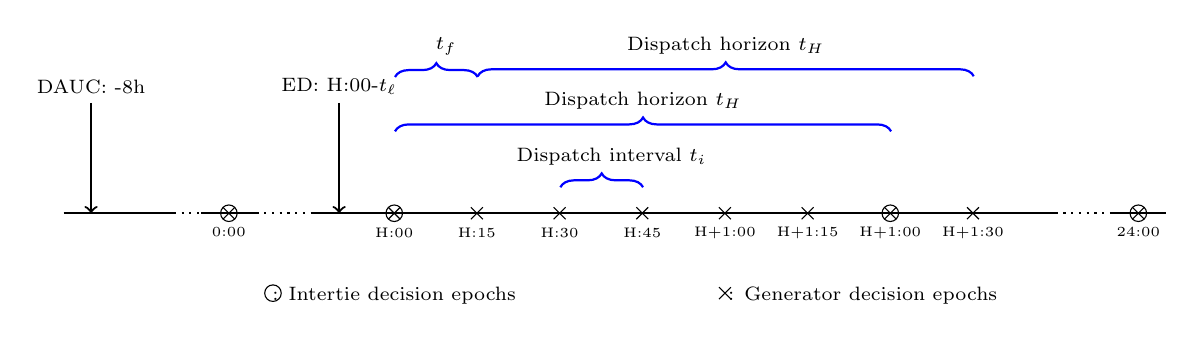
\begin{tikzpicture}[scale=0.7]
	\tikzset{cross/.style={cross out, draw=black, minimum size=2*(#1-\pgflinewidth), inner sep=0pt, outer sep=0pt}, cross/.default={0.09cm}}

	\draw[thick] (0,0) -- (2,0);
	\draw[dotted,thick] (2,0) -- (2.5,0);
	\draw[thick] (2.5,0) -- (3.5,0);
	\draw[dotted,thick] (3.5,0) -- (4.5,0);
	\draw[thick] (4.5,0) -- (18,0);
    	    \draw[dotted,thick] (18,0) -- (19,0);
	\draw[thick] (19,0) -- (20,0);

		\foreach \x in {3,6,15,19.5}{
		\draw (\x,0) circle (0.15cm);
		\draw (\x,0) node[cross] {};
	}
		
	\foreach \x in {7.5,9,10.5,12,13.5,16.5}{
		\draw (\x,0) node[cross] {};
	}
		
	\draw[->,thick] (0.5,2) -- (0.5,0);
	\node at (0.5,2.3) {\scriptsize{DAUC: -8h}};
		
	\draw[->,thick] (5,2) -- (5,0);
	\node at (5,2.3) {\scriptsize{ED: H:00-$t_{\ell}$}};

		\node at (3,-0.35) {\tiny{0:00}};
	\node at (6,-0.35) {\tiny{H:00}};
	\node at (15,-0.35) {\tiny{H+1:00}};
	\node at (19.5,-0.35) {\tiny{24:00}};

		\node at (7.5,-0.35) {\tiny{H:15}};
	\node at (9,-0.35) {\tiny{H:30}};
	\node at (10.5,-0.35) {\tiny{H:45}};
	\node at (12,-0.35) {\tiny{H+1:00}};
	\node at (13.5,-0.35) {\tiny{H+1:15}};
	\node at (16.5,-0.35) {\tiny{H+1:30}};

		\draw [thick,blue,decorate,decoration={brace,amplitude=5pt},xshift=0.4pt,yshift=-0.4pt](6,1.5) -- (15,1.5) node[black,text centered, yshift=0.6cm] at (10.5,1.2) {\scriptsize{Dispatch horizon $t_{H}$}};
	\draw [thick,blue,decorate,decoration={brace,amplitude=5pt},xshift=0.4pt,yshift=-0.4pt](7.5,2.5) -- (16.5,2.5) node[black,text centered, yshift=0.6cm] at (12,2.2) {\scriptsize{Dispatch horizon $t_{H}$}};
	\draw [thick,blue,decorate,decoration={brace,amplitude=5pt},xshift=0.4pt,yshift=-0.8pt](9,0.5) -- (10.5,0.5) node[black,text centered, yshift=0.6cm,xshift=-0.4cm] at (10.5,0.2) {\scriptsize{Dispatch interval $t_{i}$}};
	\draw [thick,blue,decorate,decoration={brace,amplitude=5pt},xshift=0.4pt,yshift=-0.8pt](6,2.5) -- (7.5,2.5) node[black,text centered, yshift=0.6cm,xshift=-0.4cm] at (7.5,2.2) {\scriptsize{$t_{f}$}};

		\draw (3.8,-1.45) circle (0.15cm);
	\node at (6,-1.5) {\scriptsize{: Intertie decision epochs}};
	\draw (12,-1.45) node[cross] {};
	\node at (14.5,-1.5) {\scriptsize{: Generator decision epochs}};
		
\end{tikzpicture}
\end{document}